%
% File: chap03.tex
% Author: Oliver J. H. Feighan
% Description: Theory and parameterization for chl-xTB method. 
% Include vibronic PES tests, and absorption spectra.
%
\let\textcircled=\pgftextcircled
\chapter{Chlorophyll specific methods}
\label{chap:chl_xtb}

\initial {P}reamble this is a preamble.

%=======
\section{The Cassida equation}
\label{sec:cassida}

\subsection{Approximations to Solutions}
\label{subsec:chl_approxs}

\subsection{MNOK Integrals}
\label{subsec:MNOK}

\section{Parameterization}
\label{sec:chl_params}

\subsection{Reference Data}
\label{subsec:ref_data}

\begin{figure}
    \includegraphics{../../Year_2/chlorophyll_parameterization/tddft_data/ResponseMethodsEnergiesCorrelations.png}
    \caption{correlations of energies}
\end{figure}

\begin{figure}
    \includegraphics{../../Year_2/chlorophyll_parameterization/tddft_data/ResponseMethodsTDMSCorrelations.png}
    \caption{correlations of transition dipole moments}
\end{figure}


\subsection{Objective Function}
\label{subsec:obj_func}

\subsection{Minimization Algorithms}
\label{subsec:algorithms}

\begin{figure}
    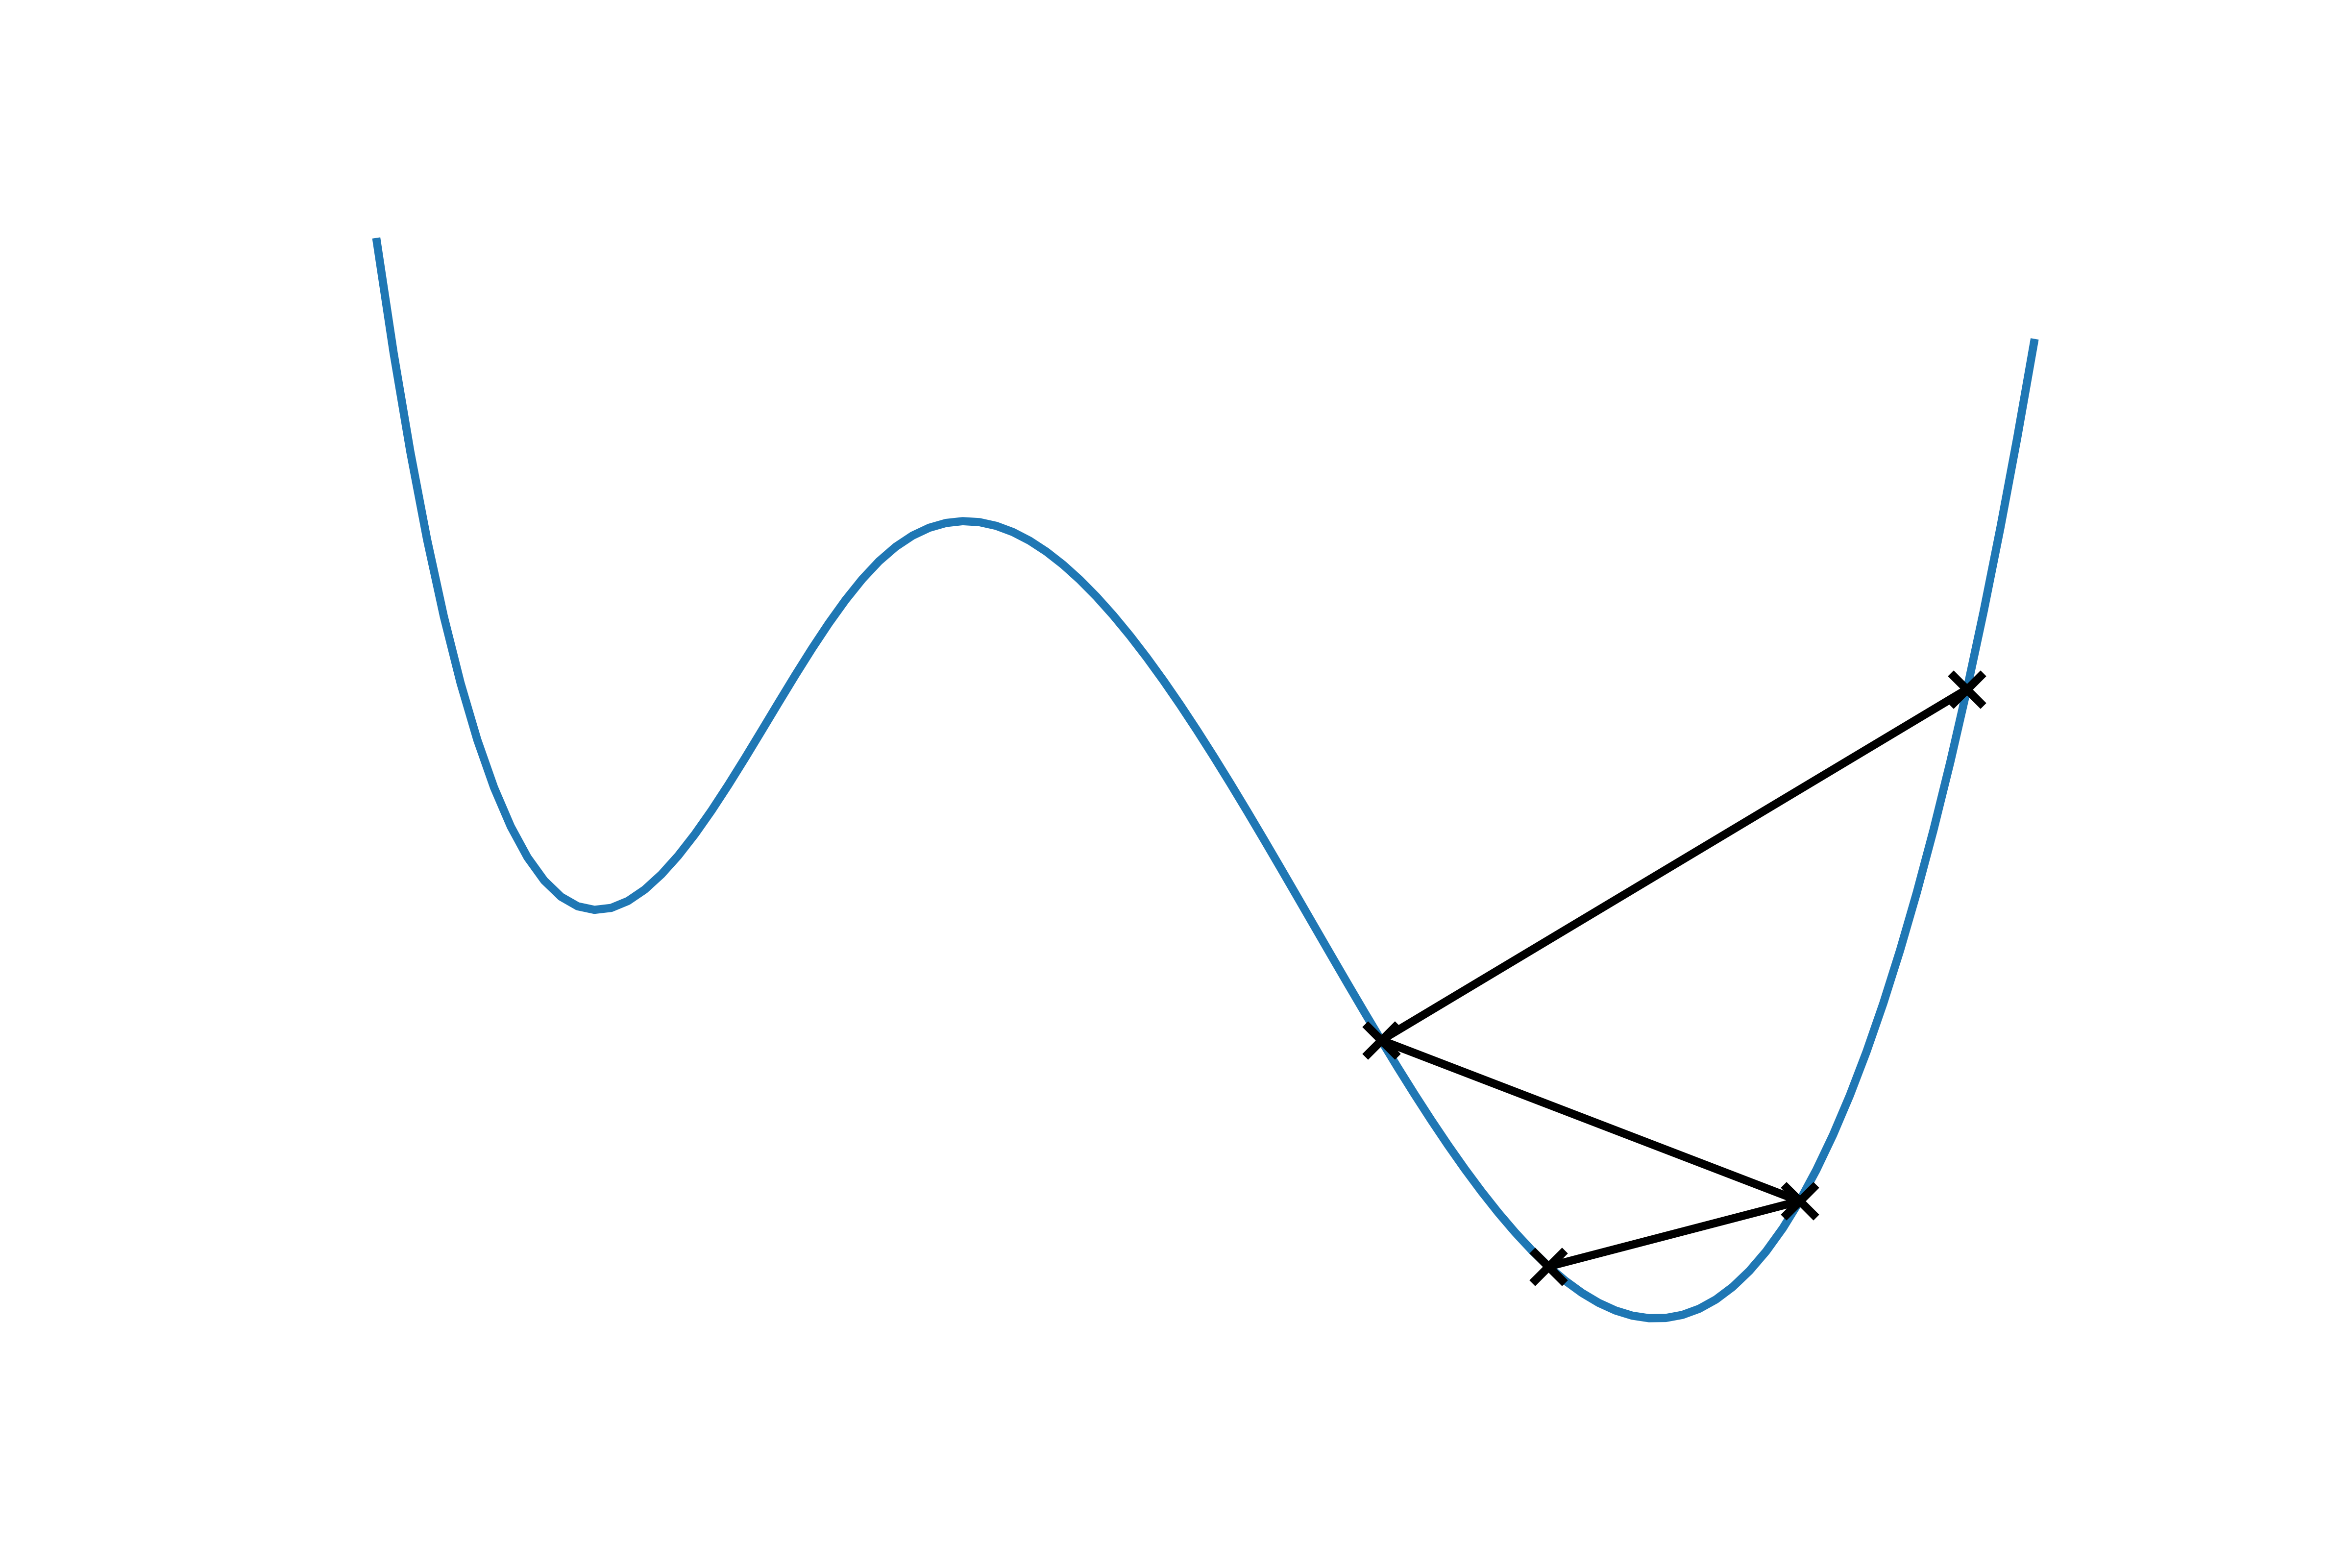
\includegraphics{nelder-mead.png}
    \caption{Nelder-mead}
\end{figure}

\begin{figure}
    \includegraphics{SLSQP.png}
    \caption{SLSQP}
\end{figure}


\begin{figure}
    \centering
    \begin{tabular}{l | r}
        \hline
        $y_K$ & 1.0 \\
        $y_J$ & 1.0 \\
        $a_x$ & 1.0 \\
        \hline
    \end{tabular}
    \caption{optimized parameters from SLSQP procedure.}
    \centering
\end{figure}

\section{Benchmarking}
\label{sec:chl_benchmarking}

\subsection{Transition properties}
\label{subsec:transition_properties}

\begin{figure}
    \includegraphics{../../Year_2/chlorophyll_parameterization/training_scatter.png}
    \caption{training scatter}
\end{figure}

\subsection{Potential Energy Surfaces}
\label{subsec:pot_energy_surfaces}

\begin{figure}
    \includegraphics{../../Year_2/BChla_Qy/Scan_of_Modes.png}
\end{figure}

\begin{figure}
    \includegraphics{../../Year_2/BChla_Qy/mode_83.png}
\end{figure}
\begin{figure}
    \includegraphics{../../Year_2/BChla_Qy/mode_85.png}
\end{figure}
\begin{figure}
    \includegraphics{../../Year_2/BChla_Qy/mode_88.png}
\end{figure}
\begin{figure}
    \includegraphics{../../Year_2/BChla_Qy/mode_90.png}
\end{figure}
\begin{figure}
    \includegraphics{../../Year_2/BChla_Qy/mode_91.png}
\end{figure}
\begin{figure}
    \includegraphics{../../Year_2/BChla_Qy/mode_129.png}
\end{figure}
\begin{figure}
    \includegraphics{../../Year_2/BChla_Qy/mode_130.png}
\end{figure}
\begin{figure}
    \includegraphics{../../Year_2/BChla_Qy/mode_132.png}
\end{figure}
\begin{figure}
    \includegraphics{../../Year_2/BChla_Qy/mode_135.png}
\end{figure}
\begin{figure}
    \includegraphics{../../Year_2/BChla_Qy/mode_162.png}
\end{figure}
\begin{figure}
    \includegraphics{../../Year_2/BChla_Qy/mode_169.png}
\end{figure}

\subsection{Absorption Spectra}
\label{subsec:absorption_spectra}


